%File: anonymous-submission-latex-2026.tex
% \documentclass[letterpaper]{article} % DO NOT CHANGE THIS
% \usepackage[submission]{aaai2026}  % DO NOT CHANGE THIS
% \usepackage{times}  % DO NOT CHANGE THIS
% \usepackage{helvet}  % DO NOT CHANGE THIS
% \usepackage{courier}  % DO NOT CHANGE THIS
% \usepackage[hyphens]{url}  % DO NOT CHANGE THIS
% \usepackage{graphicx} % DO NOT CHANGE THIS
% \urlstyle{rm} % DO NOT CHANGE THIS
% \def\UrlFont{\rm}  % DO NOT CHANGE THIS
% \usepackage{natbib}  % DO NOT CHANGE THIS AND DO NOT ADD ANY OPTIONS TO IT
% \usepackage{caption} % DO NOT CHANGE THIS AND DO NOT ADD ANY OPTIONS TO IT
\frenchspacing  % DO NOT CHANGE THIS
\setlength{\pdfpagewidth}{8.5in} % DO NOT CHANGE THIS
\setlength{\pdfpageheight}{11in} % DO NOT CHANGE THIS
%
% These are recommended to typeset algorithms but not required. See the subsubsection on algorithms. Remove them if you don't have algorithms in your paper.
% \usepackage{algorithm}
% \usepackage{algorithmic}
% \usepackage{amssymb}
% \usepackage{amsmath}
% \usepackage{xcolor}
% \newcommand{\pl}[1]{\textcolor{blue}{#1}}

% \usepackage{multirow} 
% \usepackage{booktabs}
% \usepackage{xspace}
% \usepackage{pifont}
% \newcommand{\NAMEfem}{Multi-View State-Space Enhancement Module\xspace}
% \newcommand{\NAMEdeg}{Generalized Degradation Learner\xspace}
% \newcommand{\NAMEall}{RobustGS\xspace}

% %
% % These are are recommended to typeset listings but not required. See the subsubsection on listing. Remove this block if you don't have listings in your paper.
% \usepackage{newfloat}
% \usepackage{listings}
% \DeclareCaptionStyle{ruled}{labelfont=normalfont,labelsep=colon,strut=off} % DO NOT CHANGE THIS
% \lstset{%
% 	basicstyle={\footnotesize\ttfamily},% footnotesize acceptable for monospace
% 	numbers=left,numberstyle=\footnotesize,xleftmargin=2em,% show line numbers, remove this entire line if you don't want the numbers.
% 	aboveskip=0pt,belowskip=0pt,%
% 	showstringspaces=false,tabsize=2,breaklines=true}
% \floatstyle{ruled}
% \newfloat{listing}{tb}{lst}{}
% \floatname{listing}{Listing}
% %
% % Keep the \pdfinfo as shown here. There's no need
% % for you to add the /Title and /Author tags.
% \pdfinfo{
% /TemplateVersion (2026.1)
% }


% DISALLOWED PACKAGES
% \usepackage{authblk} -- This package is specifically forbidden
% \usepackage{balance} -- This package is specifically forbidden
% \usepackage{color (if used in text)
% \usepackage{CJK} -- This package is specifically forbidden
% \usepackage{float} -- This package is specifically forbidden
% \usepackage{flushend} -- This package is specifically forbidden
% \usepackage{fontenc} -- This package is specifically forbidden
% \usepackage{fullpage} -- This package is specifically forbidden
% \usepackage{geometry} -- This package is specifically forbidden
% \usepackage{grffile} -- This package is specifically forbidden
% \usepackage{hyperref} -- This package is specifically forbidden
% \usepackage{navigator} -- This package is specifically forbidden
% (or any other package that embeds links such as navigator or hyperref)
% \indentfirst} -- This package is specifically forbidden
% \layout} -- This package is specifically forbidden
% \multicol} -- This package is specifically forbidden
% \nameref} -- This package is specifically forbidden
% \usepackage{savetrees} -- This package is specifically forbidden
% \usepackage{setspace} -- This package is specifically forbidden
% \usepackage{stfloats} -- This package is specifically forbidden
% \usepackage{tabu} -- This package is specifically forbidden
% \usepackage{titlesec} -- This package is specifically forbidden
% \usepackage{tocbibind} -- This package is specifically forbidden
% \usepackage{ulem} -- This package is specifically forbidden
% \usepackage{wrapfig} -- This package is specifically forbidden
% DISALLOWED COMMANDS
% \nocopyright -- Your paper will not be published if you use this command
% \addtolength -- This command may not be used
% \balance -- This command may not be used
% \baselinestretch -- Your paper will not be published if you use this command
% \clearpage -- No page breaks of any kind may be used for the final version of your paper
% \columnsep -- This command may not be used
% \newpage -- No page breaks of any kind may be used for the final version of your paper
% \pagebreak -- No page breaks of any kind may be used for the final version of your paperr
% \pagestyle -- This command may not be used
% \tiny -- This is not an acceptable font size.
% \vspace{- -- No negative value may be used in proximity of a caption, figure, table, section, subsection, subsubsection, or reference
% \vskip{- -- No negative value may be used to alter spacing above or below a caption, figure, table, section, subsection, subsubsection, or reference

\setcounter{secnumdepth}{0} %May be changed to 1 or 2 if section numbers are desired.

% The file aaai2026.sty is the style file for AAAI Press
% proceedings, working notes, and technical reports.
%

% Title

% Your title must be in mixed case, not sentence case.
% That means all verbs (including short verbs like be, is, using,and go),
% nouns, adverbs, adjectives should be capitalized, including both words in hyphenated terms, while
% articles, conjunctions, and prepositions are lower case unless they
% directly follow a colon or long dash
\title{RobustGS: Unified Boosting of Feedforward 3D Gaussian Splatting under Low-Quality Conditions}
\author{
    %Authors
    % All authors must be in the same font size and format.
    Written by AAAI Press Staff\textsuperscript{\rm 1}\thanks{With help from the AAAI Publications Committee.}\\
    AAAI Style Contributions by Pater Patel Schneider,
    Sunil Issar,\\
    J. Scott Penberthy,
    George Ferguson,
    Hans Guesgen,
    Francisco Cruz\equalcontrib,
    Marc Pujol-Gonzalez\equalcontrib
}
% \affiliations{
%     %Afiliations
%     \textsuperscript{\rm 1}Association for the Advancement of Artificial Intelligence\\
%     % If you have multiple authors and multiple affiliations
%     % use superscripts in text and roman font to identify them.
%     % For example,

%     % Sunil Issar\textsuperscript{\rm 2},
%     % J. Scott Penberthy\textsuperscript{\rm 3},
%     % George Ferguson\textsuperscript{\rm 4},
%     % Hans Guesgen\textsuperscript{\rm 5}
%     % Note that the comma should be placed after the superscript

%     1101 Pennsylvania Ave, NW Suite 300\\
%     Washington, DC 20004 USA\\
%     % email address must be in roman text type, not monospace or sans serif
%     proceedings-questions@aaai.org
% %
% % See more examples next
% }

%Example, Single Author, ->> remove \iffalse,\fi and place them surrounding AAAI title to use it
\iffalse
\title{My Publication Title --- Single Author}
\author {
    Author Name
}
\affiliations{
    Affiliation\\
    Affiliation Line 2\\
    name@example.com
}
\fi

\iffalse
%Example, Multiple Authors, ->> remove \iffalse,\fi and place them surrounding AAAI title to use it
\title{My Publication Title --- Multiple Authors}
\author {
    % Authors
    First Author Name\textsuperscript{\rm 1},
    Second Author Name\textsuperscript{\rm 2},
    Third Author Name\textsuperscript{\rm 1}
}
\affiliations {
    % Affiliations
    \textsuperscript{\rm 1}Affiliation 1\\
    \textsuperscript{\rm 2}Affiliation 2\\
    firstAuthor@affiliation1.com, secondAuthor@affilation2.com, thirdAuthor@affiliation1.com
}
\fi


% REMOVE THIS: bibentry
% This is only needed to show inline citations in the guidelines document. You should not need it and can safely delete it.
% \usepackage{bibentry}
% % END REMOVE bibentry

% \begin{document}

\maketitle


\section{Implementation Details}

The training process consists of two stages. In the first stage, we use the DIV2K dataset as the source of high-quality (HQ) images and generate their corresponding low-quality (LQ) versions using the same degradation method as in RobustSAM ~\cite{chen2024robustsam}. The degradation types used during training include dark, fog, rain, snow, high contrast, and impulse noise. We train \NAMEdeg (GenDeg) for 20{,}000 iterations. 
In the second stage, we randomly select two HQ frames from each video sequence and generate their corresponding LQ frames using the same degradation strategy as in the first stage. The two LQ frames are passed through the pretrained feature extraction network provided by PixelSplat or other feedforward 3DGS backbone to obtain feature maps. These feature maps, along with their corresponding degradation embeddings extracted by the pretrained GenDeg, are then fed into \NAMEfem (MV-SSEM) for enhancement. During this stage, GenDeg functions solely as a fixed degradation extractor, with its parameters frozen and excluded from the training process. The enhanced feature maps are supervised using the L1 loss function. Adam~\cite{kingma2014adam} is used as the optimizer, with the initial learning rate set to 1e-4 and halved every 100 epochs. The model is trained for 1000 epochs with a total batch size of 32 on 8 NVIDIA 4090 GPUs.


\section{Algorithm Workflow}

To clearly demonstrate the details of the proposed semantic-guided mechanism, we design an algorithm workflow, as illustrated in Algorithm~\ref{alg:semantic}. It outlines the entire process from multi-view feature flattening to token-level semantic assignment, reordering, prompt generation, and final enhancement via selective scan modulation. This mechanism plays a central role in enabling semantic-aware feature aggregation and enhancement across views.


% \begin{algorithm}[t]
% \caption{Semantic-guided mechanism}
% \begin{algorithmic}[1]
% \REQUIRE $x \in \mathbb{R}^{B \times V \times C \times H \times W}$ \hfill // multi-view features
% % \REQUIRE $z \in \mathbb{R}^{B \times V \times 256 \times 1 \times 1}$ (optional)
% \ENSURE $\texttt{prompt\_sorted} \in \mathbb{R}^{B \times L \times d_{\text{state}}} , \texttt{x\_sorted} $

% \STATE $L \gets V \cdot H \cdot W$
% \STATE $x_{\text{seq}} \gets \text{reshape}(x, [B, L, C])$ \hfill // flatten token sequence

% \STATE $q \gets \text{MLP}(x_{\text{seq}}) \in \mathbb{R}^{B \times L \times d_{\text{inner}}}$ \hfill // token query
% \STATE $K \gets \text{PromptPool} \in \mathbb{R}^{T \times d_{\text{inner}}}$ \hfill // prompt keys


% \STATE $P \gets \text{GumbelSoftmax}(r)$ \hfill // one-hot class distribution

% \STATE $\texttt{class\_id} \gets \arg\max(P) \in \mathbb{R}^{B \times L}$
% \STATE $\texttt{sort\_idx} \gets \texttt{argsort}(\texttt{class\_id})$

% \STATE $E \gets P \cdot K \in \mathbb{R}^{B \times L \times d_{\text{inner}}}$
% \STATE $\texttt{prompt} \gets \text{Linear}(E) \in \mathbb{R}^{B \times L \times d_{\text{state}}}$

% \STATE $\texttt{x\_sorted} \gets \texttt{gather}(x_{\text{seq}}, \texttt{sort\_idx})$
% \STATE $\texttt{prompt\_sorted} \gets \texttt{gather}(\texttt{prompt}, \texttt{sort\_idx})$

% \RETURN $\texttt{prompt\_sorted, x\_sorted}$ 
% \end{algorithmic}
% \end{algorithm}

\begin{algorithm}[t]
\caption{Semantic-Guided Mechanism}
\begin{algorithmic}[1]
\REQUIRE $x \in \mathbb{R}^{B \times V \times C \times H \times W}$ \hfill // multi-view features
\ENSURE ${\mathbf{x}}^\text{enhanced} \in \mathbb{R}^{B \times L \times C}$

\STATE $L \gets V \cdot H \cdot W$
\STATE $\mathbf{x} \gets \text{reshape}(x, [B, L, C])$ \hfill // flatten tokens
\STATE $\mathbf{q} \gets \text{MLP}(\mathbf{x})$ \hfill // token-wise semantic query
\STATE $\mathbf{r} \gets \text{Linear}(\mathbf{q}) \in \mathbb{R}^{B \times L \times T}$ \hfill // logits for routing to $T$ semantic prompts
\STATE $\mathbf{P} \gets \text{GumbelSoftmax}(\mathbf{r}, \text{dim}=T)$ \hfill // hard one-hot token assignment

\STATE $c \gets \arg\max(\mathbf{P}, \text{dim}=T)$ \hfill // prompt class index per token
\STATE $\pi \gets \text{argsort}(c)$ \hfill // sort tokens by assigned prompt class

\STATE $\mathbf{e} \gets \mathbf{P} \cdot \mathbf{W}_E$ \hfill // embedding lookup from prompt pool
\STATE $\mathbf{p} \gets \text{Linear}(\mathbf{e})$ \hfill // semantic prompt per token

\STATE $\mathbf{x}' \gets \text{gather}(\mathbf{x}, \pi)$ \hfill // token reordering
\STATE $\mathbf{p}' \gets \text{gather}(\mathbf{p}, \pi)$

\STATE $\hat{\mathbf{x}} \gets \text{SelectiveScan}(\mathbf{x}', \mathbf{p}')$ \hfill // SSM modulated by semantic prompt

\STATE $\pi^{-1} \gets \text{inverse\_argsort}(\pi)$ \hfill // recover original order
\STATE ${\mathbf{x}}^{\text{enhanced}} \gets \text{gather}(\hat{\mathbf{x}}, \pi^{-1})$

\RETURN ${\mathbf{x}}^\text{enhanced}$
\end{algorithmic}
\label{alg:semantic}
\end{algorithm}





\section{Addtional Comparison}
\subsection{More Results of Mvsplat}
In the main paper, we have compared our proposed method based on PixelSplat under six different types of degradations. We also reported the average performance over multiple degradations on MVSplat. As shown in Table~\ref{table_mvsplat}, we further present detailed performance comparisons on MVSplat under each individual degradation type.

\begin{table*}[ht]
\centering
\setlength{\tabcolsep}{1.5mm}
\begin{tabular}{l|ll|ll|ll|ll|ll|ll}
\toprule
         & \multicolumn{2}{c|}{Brightness}   & \multicolumn{2}{c|}{Fog}          & \multicolumn{2}{c|}{Rain}        & \multicolumn{2}{c|}{Snow}         & \multicolumn{2}{c|}{Contrast}     & \multicolumn{2}{c}{Impulse noise} \\
         \cmidrule(lr){2-13}
         & PSNR           & SSIM            & PSNR           & SSIM            & PSNR          & SSIM            & PSNR           & SSIM            & PSNR           & SSIM            & PSNR            & SSIM            \\
          \midrule
mvsplat  & 15.58          & 0.8035          & 15.52          & 0.7471          & 19.97         & 0.7498          & 19.17          & 0.5852          & 18.51          & 0.7298          & 14.47           & 0.7688          \\
PromptIR & 14.87          & 0.7791          & \textbf{21.52} & \textbf{0.8432} & 21.99         & 0.7637          & 19.93          & 0.6216          & 18.39          & 0.7262          & 14.70           & 0.7732          \\
PromptI\ding{72} & 16.45          & 0.7722          & 20.47          & 0.8048          & 21.02         & 0.7765          & \textbf{21.52} & \textbf{0.6807} & \underline{20.95}    & \underline{0.7704}    & 19.84           & 0.7908          \\
PromptIR\ding{73} & 17.34          & 0.7703          & 20.78          & 0.8129          & 20.09         & 0.7546          & 19.22          & 0.6234          & 18.17          & 0.7274          & 20.26           & 0.7970          \\
AdaIR    & 15.37          & 0.7950          & \underline{20.95}    & \underline{0.8329}    & 21.37         & 0.7560          & 19.74          & 0.6171          & 18.43          & 0.7285          & 14.73           & 0.7702          \\
AdaIR\ding{72}    & 21.74          & \underline{0.8460}     & 15.95          & 0.7476          & \underline{22.23}   & \underline{0.7839}    & 17.58          & 0.6387          & 19.43          & 0.7412          & \underline{20.57}     & 0.8029          \\
AdaIR\ding{73}    & \underline{22.05}    & 0.8455          & 16.93          & 0.7250          & 19.91         & 0.7689          & 15.30          & 0.6005          & 15.36          & 0.6826          & 20.28           & \underline{0.8063}    \\
RobustGS & \textbf{22.56} & \textbf{0.8481} & 20.63          & 0.8179          & \textbf{22.50} & \textbf{0.7858} & \underline{21.10}     & \underline{0.6664}    & \textbf{21.09} & \textbf{0.7853} & \textbf{21.01}  & \textbf{0.8071}
\\ \bottomrule
\end{tabular}
\caption{Comparison of performance on Mvsplat with existing methods across various degradation scenarios. Bold indicates the best performance, while underline denotes the second-best.}
\label{table_mvsplat}
\end{table*}


\subsection{Additional Visual Comparison Results}
In this section, we present additional visual comparison results on novel view synthesis to further demonstrate the superiority of our proposed method, as shown in Figure~\ref{fig:vis_rgb}. It can be observed that our method achieves the best visual satisfaction in terms of detailed textures, while also preserving the highest level of detail fidelity, making it closest to the GT image.

\begin{figure*}[t]
\centering
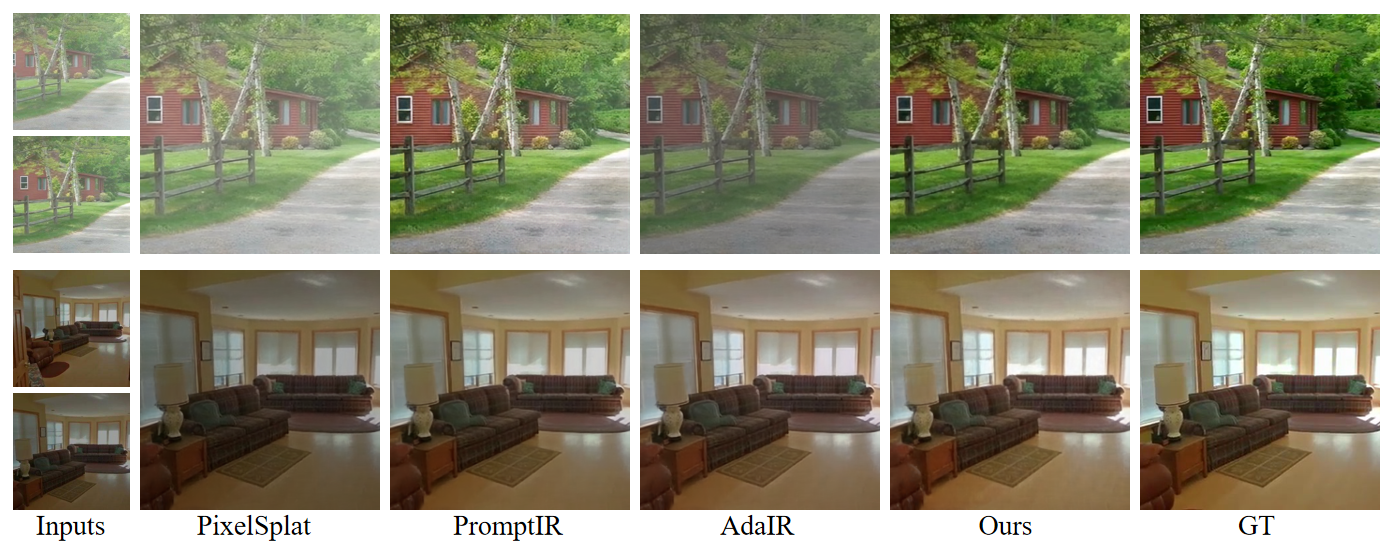
\includegraphics[width=1.0\textwidth]{fig_sup.png} % Reduce the figure size so that it is slightly narrower than the column. Don't use precise values for figure width.This setup will avoid overfull boxes.
\caption{Additional qualitative comparison. The visual quality of our method outperforms restore before reconstruct methods. Visual examples in the first and second rows correspond to foggy and dark degradation scenes, respectively.}
\label{fig:vis_rgb}
\end{figure*}

\section{Additional Ablation Study}
Due to space limitations in the main text, we provide additional ablation experiments to demonstrate the effectiveness and rationality of the proposed method. Below, we present detailed descriptions of additional ablation studies and implementation details.

\paragraph{Ablation Study on GenDeg.}
Existing methods such as DegAE adopt a degradation-aware encoder to extract degradation embeddings from input images for restoration purposes, but these approaches typically rely on reconstruction loss alone. In contrast, our proposed GenDeg introduces two additional objectives: a contrastive loss to encourage discrimination between different degradation types and a classification loss to further promote semantic alignment with known degradation categories. Table~\ref{table_deg} presents an ablation study on the loss functions used in GenDeg, demonstrating that our design contribute significantly to performance.

\begin{table}[th!]
\centering
\begin{tabular}{ccc|ll}
\toprule
$\mathcal{L}_{\mathrm{rec}}$ & $\mathcal{L}_{\mathrm{con}}$ & $\mathcal{L}_{\mathrm{cls}}$ & PSNR  & SSIM   \\ \midrule
\checkmark                   &                  &                     & 21.87 & 0.7751 \\
\checkmark                   & \checkmark                &                     & 22.09 & 0.7816 \\
\checkmark                   &                  & \checkmark                   & 21.95 & 0.7810  \\
\checkmark                   & \checkmark                & \checkmark                   & 22.32 & 0.7869
\\ \bottomrule
\end{tabular}
\caption{Ablation study on training loss of GenDeg.}
\label{table_deg}
\end{table}


\paragraph{Ablation Study on MV-SSEM.}
In the MV-SSEM, we use a semantic prompt pool of size $K$ to cluster tokens based on semantic similarity. We conduct an ablation study by varying the number of semantic prompts ($K=32, 64, 128$), as shown in Table~\ref{tab:prompt_k}. The results indicate that $K=64$ yields the best performance. A smaller $K$ leads to overly coarse semantic grouping, while a larger $K$ causes excessive fragmentation, making cross-view aggregation unstable. These experientments validate our design choice for prompt pool size.

We also conduct an ablation study to evaluate the impact of the internal dimensionality of each semantic prompt, denoted as $d_{\text{inner}}$, on the final performance. As shown in Table~\ref{tab:prompt_dim}, increasing the dimensionality from 32 to 128 leads to consistent improvements. However, further increasing beyond 128 brings no significant gain. Therefore, we choose $d_{\text{inner}} = 128$ in our implementation to balance representation capacity and computational cost.

\begin{table}[ht]
\centering
\begin{tabular}{c|ccc}
\toprule
Prompt Number ($K$) & PSNR & SSIM  & LPIPS \\
\midrule
32  & 21.93 & 0.7804 & 0.2513 \\
128 & 21.75 & 0.7717 & 0.2488 \\
64  & \textbf{22.32} & \textbf{0.7869} & \textbf{0.2443} \\
\bottomrule
\end{tabular}
\caption{Ablation study on $K$. }
\label{tab:prompt_k}
\end{table}

\begin{table}[ht]
\centering
\begin{tabular}{c|ccc}
\toprule
Prompt Dim ($d_{\text{inner}}$) & PSNR & SSIM  & LPIPS \\
\midrule
32   & 21.95 & 0.7798 & 0.2564 \\
64   & 22.24 & 0.7847 & 0.2471 \\
128  & \textbf{22.32} & \textbf{0.7869} & \textbf{0.2443} \\
\bottomrule
\end{tabular}
\caption{Ablation on $d_{\text{inner}}$.}
\label{tab:prompt_dim}
\end{table}


% \bibliography{aaai2026}

% \end{document}